\documentclass{article}

\usepackage[english]{babel} %Forces American English hyphenation patters
\usepackage[utf8x]{inputenc} % Unicode
\usepackage{amsmath, amssymb, amsthm, mathtools} %Math Packages
\usepackage{textcomp, siunitx, gensymb, wasysym} %Symbol Packages
\usepackage{multicol, geometry, fancyhdr, enumitem} %Page Layout Packages 
\usepackage{graphicx, wrapfig, subcaption} %Figure Packages
\usepackage{hyperref}

\newcommand{\Lim}[1]{\underset{#1}{\lim}}
\newcommand{\vvert}[1]{\left \lvert #1 \right \rvert}
\newcommand{\vVert}[1]{\left \lVert #1 \right \rVert}
\newcommand{\Rom}[1]{\MakeUppercase{\romannumeral #1}}
\newcommand{\rom}[1]{\romannumeral #1}
\renewcommand{\l}{\left}
\renewcommand{\r}{\right}
\newcommand{\reals}{\mathbb{R}}
\newcommand{\rationals}{\mathbb{Q}}
\newcommand{\naturals}{\mathbb{N}}
\newcommand{\integers}{\mathbb{Z}}
\newcommand{\complex}{\mathbb{C}}


\hypersetup{colorlinks=true, urlcolor = blue, linkcolor=black}
\graphicspath{ {./Images/} }
\geometry{margin = 1in}
\setlength{\parindent}{0pt}

\pagestyle{fancyplain}
\headheight 1cm
\lhead{Michael Dymek \\ May 7, 2022}
\chead{\textbf{\Large Omicron Modeling Project}}
\rhead{Dr. Tilmann Glimm \\ Mathematical Epidemiology}
\headsep .5cm

\begin{document}
\textbf{Project Description: }This project concerns the Omicron wave in Washington state. I have included the official data for hospitalization in Washington State. Assume that hospitalizations due to COVID are proportional to the number of COVID cases; the proportionality coefficent is the probability that a COVID infections leads to hospitalizations. (This was estimated to be around 2.8\% for the Omicron variant for unvaccinated individuals and lower for vaccinated individuals.) One difficulty is that at that point, the population was not immunologically naive – many were vaccinated, some had recovered from an infection with another variant or both. \medskip

Fit an SIR model and an SEIR model to the hospitalization data from December 14, 2021 to April 18, 2022. Compute Aikaike Information Criterion for the two models. Discuss your findings. For extra credit, set up a more sophisticated model that takes into account two or more population groups – e.g. vaccinated versus unvaccinated.
\medskip

\textbf{Solution: }For this problem, we will fit the SIR, SEIR, and SVIR. Our SIR model is given by
\[ S' = -\beta SI, ~~~~~~~~ I' = \beta SI - \alpha I, ~~~~~~~~ R' = \alpha I, \]
our SEIR model is given by
\[ S' = -\beta SI, ~~~~~~~~E' = \beta SI - \eta E,~~~~~~~~ I' = \eta E - \alpha I, ~~~~~~~~ R' = \alpha I, \]
and our SVIR model is given by 
\[ S' = -\beta SI-\psi S, ~~~~~~~~V' = \psi S - \delta \beta VI,~~~~~~~~ I' = \beta SI + \delta \beta VI - \alpha I, ~~~~~~~~ R' = \alpha I. \]
From the data, we've isolated just the data for the omicron wave, which represents data between 12/14/2021 and 04/18/2022, coming out to 126 total data points. Since this data is only accounting for the hospitalized individuals, we will divide the data by $2.8\%=0.028$, which is the approximate proportion of infected individuals who become hospitalized. This roughly converts our hospitalization data into total infections. We will use some Matlab code to fit the parameters in these models, and compute the Aikaike Information Criterion. Since the SVIR has 4 parameters, and $\frac{126}{4} = 31.5 < 40$, we will actually want to use the Corrected Akeike Information Criterion so that we can compare all the models appropriately:
\[ AIC_{c} = n \ln \l( \frac{SEE}{n} \r) + 2k + \frac{2k(k-1)}{n-k-1}. \]
If Figure \ref{fig:Modeling_Problem_Fitted_Plots}, the plots of each of the models, along with the computed parameters and $AIC_c$ values, are shown. Since the SEIR model has the smallest $AIS_c$ value, we can set $AIC_{\text{min}} = 2.4557\times 10^{3}$. Then, with $\Delta AIC_j = AIC_j - AIC_{\text{min}}$, we calculate
\[ \Delta AIC_1 = 165.8,~~~~\Delta AIC_2 = 0, ~~~~ \Delta AIC_3 = 170.7. \]
The weights then become 
\begin{align*}
    w_{SIR} = \frac{e^{-(\Delta AIC_{1}/2}}{e^{-(\Delta AIC_{1}/2}+e^{-(\Delta AIC_{2}/2}+e^{-(\Delta AIC_{3}/2}} \approx 0, \\
    w_{SEIR} = \frac{e^{-(\Delta AIC_{2}/2}}{e^{-(\Delta AIC_{1}/2}+e^{-(\Delta AIC_{2}/2}+e^{-(\Delta AIC_{3}/2}} \approx 1, \\
    w_{SVIR} = \frac{e^{-(\Delta AIC_{3}/2}}{e^{-(\Delta AIC_{1}/2}+e^{-(\Delta AIC_{2}/2}+e^{-(\Delta AIC_{3}/2}} \approx 0.
\end{align*}
Since the weights associated with the SIR and SVIR models are so small, and the weight associated with the SEIR model is so large, we can conclude that the SEIR model is all we need out of the three options to accurately model the data.

\begin{figure}[ht]
    \centering
    \begin{subfigure}{0.32\textwidth}
        \centering
        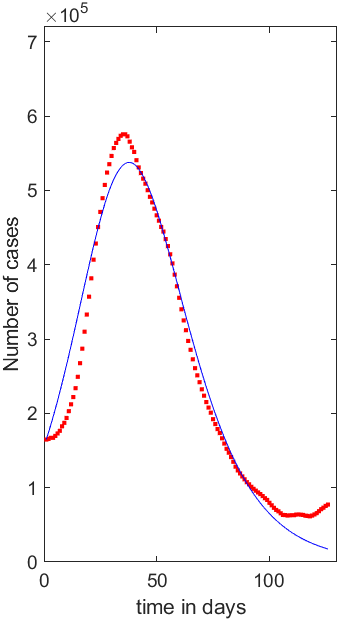
\includegraphics[width = \textwidth]{Images/Modeling_Problem_SIR_Model.png}
        \subcaption{SIR Model fitted to the given Omicron wave data. The fitted parameters are $\alpha = 0.1353$ and $\beta = 2.5287\times 10^{-8}$. The Aikaike Information Criterion is $AIC_{c} = 2.6215\times 10^{3}$.}
        \label{sfig:Modeling_Problem_SIR_Model}
    \end{subfigure}
    \hfill
    \begin{subfigure}{0.32\textwidth}
        \centering
        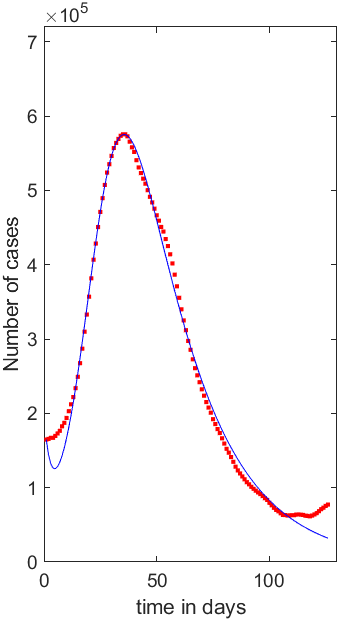
\includegraphics[width = \textwidth]{Images/Modeling_Problem_SEIR_Model.png}
        \subcaption{SEIR Model fitted to the given Omicron wave data. The fitted parameters are $\alpha = 0.1567$, $\beta = 2.3452\times 10^{-7}$ and $\eta = 0.03676$. The Aikaike Information Criterion is $AIC_{c} = 2.4557\times 10^{3}$.}
        \label{sfig:Modeling_Problem_SEIR_Model}
    \end{subfigure}
    \hfill
    \begin{subfigure}{0.32\textwidth}
        \centering
        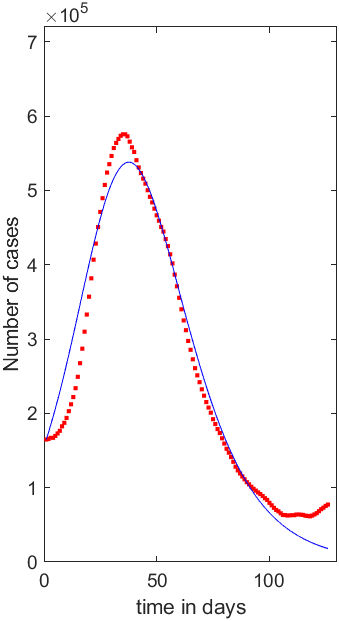
\includegraphics[width = \textwidth]{Images/Modeling_Problem_SVIR_Model.png}
        \subcaption{SVIR Model fitted to the given Omicron wave data. The fitted parameters are $\alpha = 0.1325$, $\beta = 3.3412\times 10^{-8}$, $\psi = 1.4917\times 10^{-11}$ and $\delta = 0.6381$. The Aikaike Information Criterion is $AIC_{c} = 2.6264\times 10^{3}$.}
        \label{sfig:Modeling_Problem_SVIR_Model}
    \end{subfigure}
    \caption{Models of the Omicron wave for the SIR, SEIR, and SVIR models. The computed parameter values and $AIC_c$ values included.}
    \label{fig:Modeling_Problem_Fitted_Plots}
\end{figure}
\newpage


\end{document}